% 2D Distance from Point to Line Segment Two
%
% File:         2d-point-to-line-segment-2.tex
% Author:       Bob Walton (walton@acm.org)
% Date:      	Tue Dec 25 17:56:40 EST 2012
  
\documentclass{minimal}
\usepackage[paperheight=2.8in,paperwidth=2.6in,
            height=2.8in,hoffset=0in,
	    voffset=0.05in,left=0in,width=2.6in]{geometry}
\usepackage{color}
\usepackage[usenames]{xcolor}
\usepackage{scalefnt}
\usepackage[greek,english]{babel}
\usepackage{tikz}
\newcommand{\SMALL}{\scalefont{0.8}}
\newcommand{\THETA}{{\greektext J}}
\usetikzlibrary{arrows}
\begin{document}
\raggedright
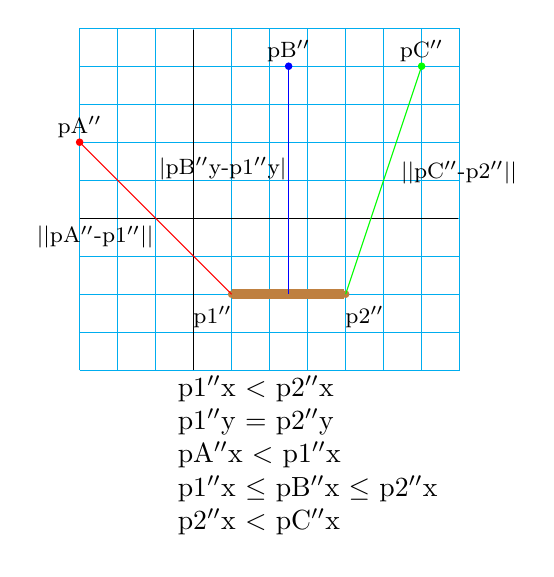
\begin{tikzpicture}[x=0.190in,y=0.190in]
\begin{scope}[yshift=1in,>=triangle 45,shorten >=0.01in]
    \draw[cyan] (-3,-4) grid[step=1] (7,5);
    \draw[black] (-3,0) -- (+7,0);
    \draw[black] (0,-4) -- (0,+5);

    \fill[brown] (1,-2) circle(0.1) + (-0.5,-0.6) node[black]{\SMALL p1$''$};
    \draw[brown,line width=0.05in] (1,-2) -- (4,-2);
    \fill[brown] (4,-2) circle(0.1) + (+0.5,-0.6) node[black]{\SMALL p2$''$};

    \fill[red] (-3,+2) circle(0.1) + (+0,+0.4) node[black]{\SMALL pA$''$};
    \draw[red] (1,-2) -- (-3,+2);
    \draw[black] (-1.0,-0.5) + (+0.2,0) node[left]{\SMALL $||$pA$''$-p1$''$$||$};

    \fill[blue] (+2.5,+4) circle(0.1) + (+0,+0.4) node[black]{\SMALL pB$''$};
    \draw[blue] (+2.5,-2) -- (+2.5,+4);
    \draw[black] (2.5,1) + (+0.2,+0.3) node[left]{\SMALL $|$pB$''$y-p1$''$y$|$};

    \fill[green] (+6,+4) circle(0.1) + (+0,+0.4) node[black]{\SMALL pC$''$};
    \draw[green] (4,-2) -- (+6,+4);
    \draw[black] (5,1) + (+0.2,+0.2) node[right]{\SMALL $||$pC$''$-p2$''$$||$};
\end{scope}

\draw[black] (3,-1) node {
    \begin{tabular}[t]{l}
    p1$''$x $<$ p2$''$x \\
    p1$''$y = p2$''$y \\
    pA$''$x $<$ p1$''$x \\
    p1$''$x $\le$ pB$''$x $\le$ p2$''$x \\
    p2$''$x $<$ pC$''$x \\
    \end{tabular}
};

\end{tikzpicture}
\end{document}




